\documentclass[twocolumn]{article}
\usepackage{url}
\usepackage{graphicx}
\usepackage{color}
\graphicspath{{./images/}}

\title{Improving Condition- and Environment-Invariant Place Recognition with Semantic Place Categorization}
\author{Author}


\begin{document}

\maketitle

\section{Abstract}
The problem of place recognition actually comprises two distinct subproblems; "ordinary" place recognition which is recognizing a specific location in the world, and place "categorization", which involves recognizing the type of place. Both components of place recognition are competencies for robotic navigation systems and hence have each in isolation received significant attention in the robotics and computer vision community. In this paper, we leverage the powerful complementary nature of the place recognition and place categorization processes to create a new state-of-the-art ordinary place recognition system that uses place context to inform place recognition. We show that semantic place categorization creates a more informative natural segmenting of physical space than the blindly applied fixed segmentation used in algorithms such as SeqSLAM, which enables significantly better place recognition performance. In particular, where existing condition-invariant algorithms enable robustness to globally consistent change (such as day to night cycles), this new semantically informed approach adds robustness to significant changes within the environment, such as transitioning from indoor to outdoor environments. We perform a number of experiments using benchmark and new datasets and show that semantically-informed place recognition outperforms the previous state of the art systems. Like it does for object recognition [ref Niko IROS2015], we believe that  semantics can play a key role in boosting conventional place recognition and navigation performance for robotic systems.

\section{Introduction}

\section{Related Work}

\section{Proposed Method}
The proposed approach has two main components: place categorization and place recognition. We use CNN model VGG16-places365 \cite{cnnPlaces365Github} pre-trained on Places365 database \cite{zhou2014learning} for labeling reference and query database images as indoor or outdoor. The place recognition is done using SeqSLAM \cite{Milford2012} and appropriate normalization of image matching scores with help of semantic image labels.

\subsection{Place Categorization}

The pre-trained CNN model classifies an image with probabilities associated with each of the 365 place categories. 205 of these place categories also have binary labels classifying an image as indoor or outdoor. We added the indoor/outdoor labels for rest of the 160 place categories. We use top-5 most probable predictions from the pre-trained model to calculate a weighted score for labeling an image as indoor or outdoor. Figure \ref{fig:labelledImages} shows images with indoor/outdoor label, top predicted place label and its associated probability.

\newcommand{\scaleVal}{0.28}
\begin{figure*}[!htbp]
 \begin{tabular*}{\textwidth}{lcr}
  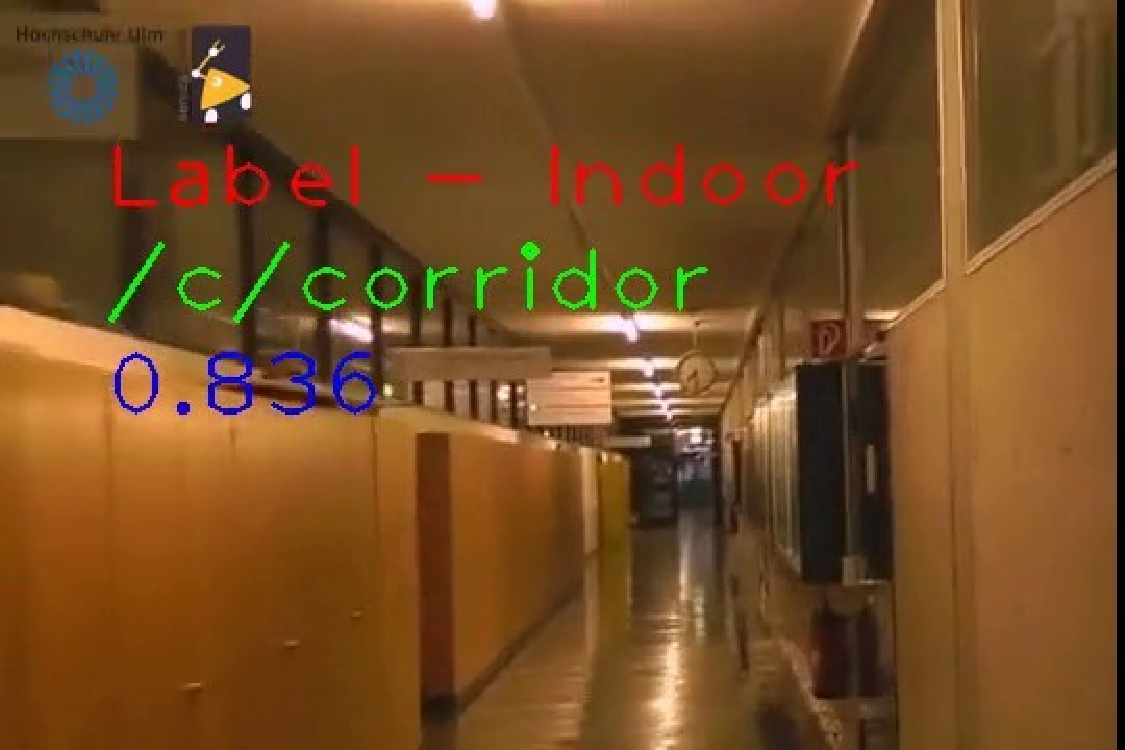
\includegraphics[scale=\scaleVal]{1-corridor} &
  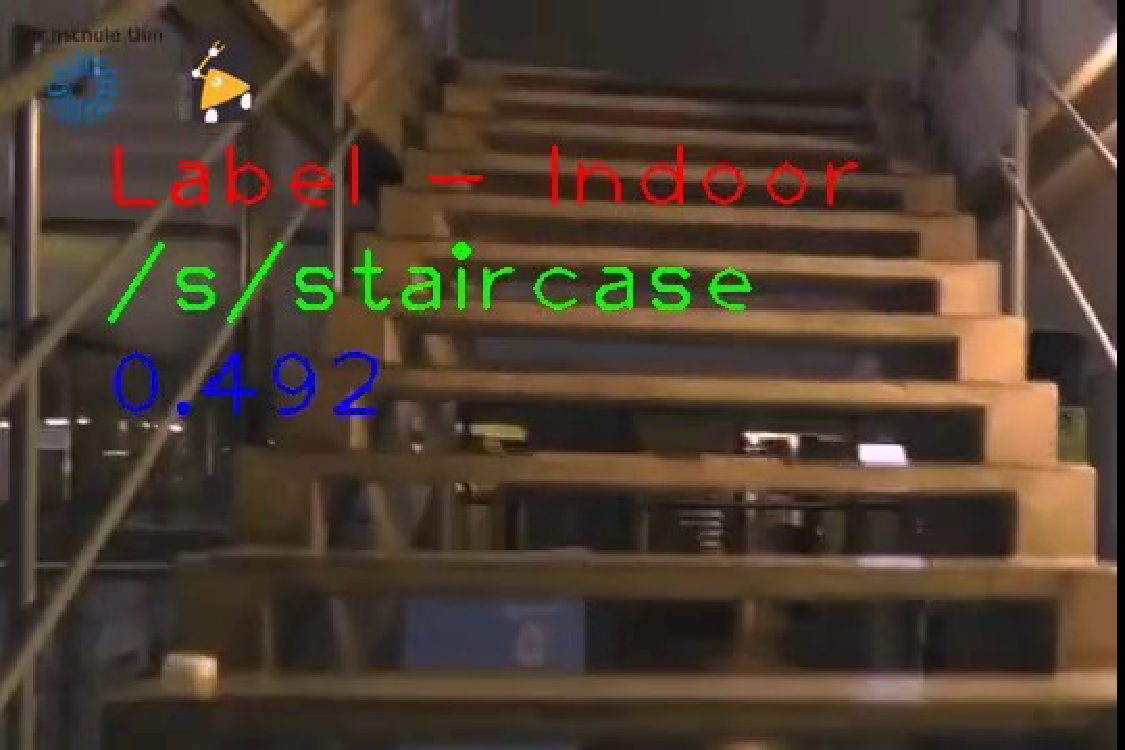
\includegraphics[scale=\scaleVal]{2-staircase} &
%  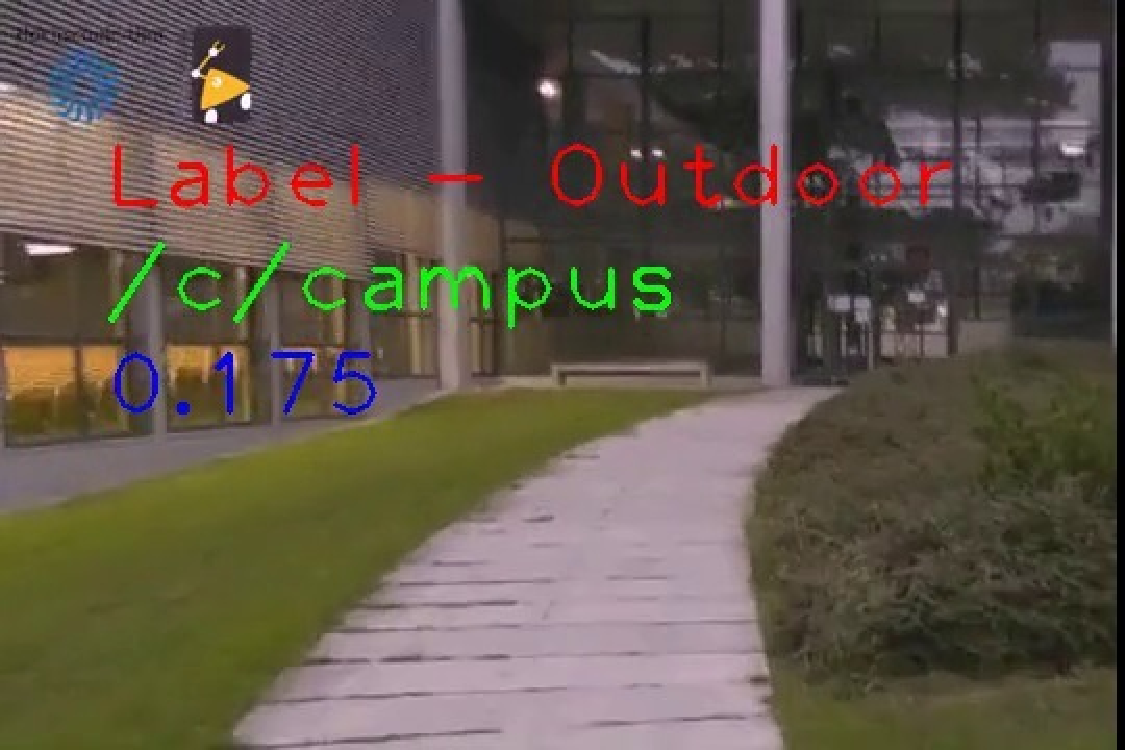
\includegraphics[scale=\scaleVal]{3-campus} &
  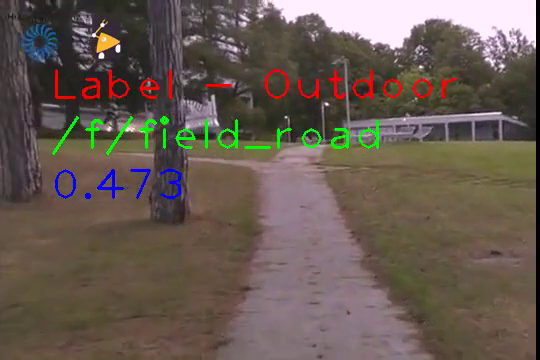
\includegraphics[scale=\scaleVal]{4-fieldRoad} \\
  & (a) & \\
%  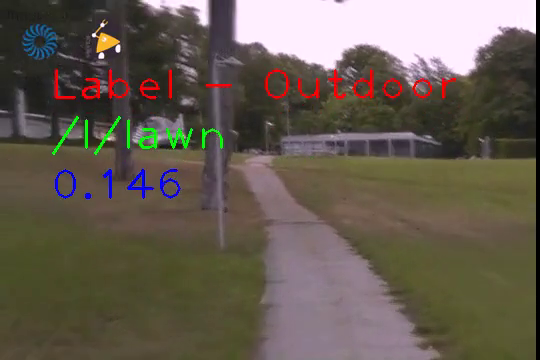
\includegraphics[scale=\scaleVal]{5-lawn} &
  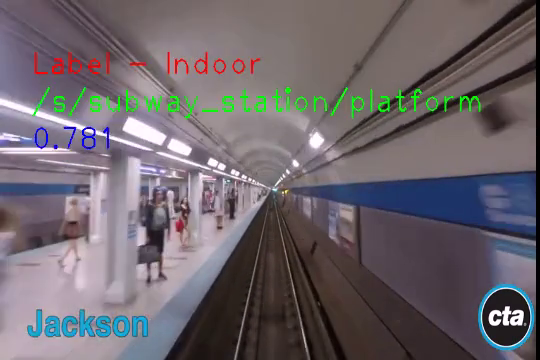
\includegraphics[scale=\scaleVal]{6-subwayStation} &
  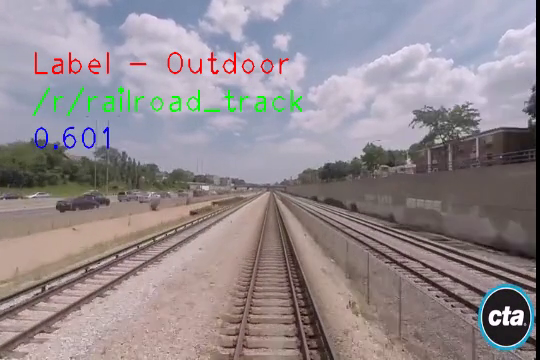
\includegraphics[scale=\scaleVal]{7-railroadTrack} &
  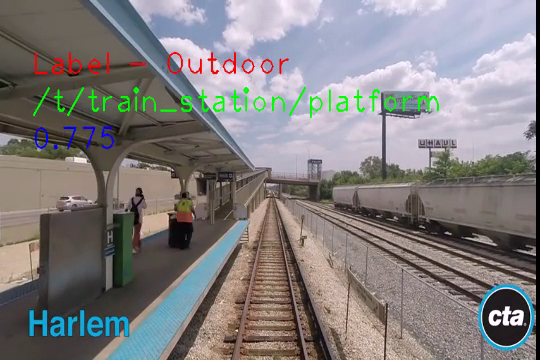
\includegraphics[scale=\scaleVal]{8-trainStation} \\
  & (b) &
 \end{tabular*}
 \caption{Images from reference database with indoor/outdoor labels, top predicted label from 365 place categories and its associated probability. (a) Campus Dataset and (b) CTA Rail Dataset}
 \label{fig:labelledImages}
\end{figure*}

The images are labeled for the entire reference and query database. These labels are then filtered using a sliding window approach over the entire image sequence. The label of an image frame is replaced by the mode of image labels in the window centered at it. Figure \ref{fig:datasetLabels} shows the final labels for reference and query database for one of the datasets used in this paper. These semantic labels show the corresponding matching environments. Though the dataset start and end point is fixed and same in both the traversals, the difference in speed of vehicle prevents perfect alignment of labels in the figure.

\begin{figure}[!htbp]
 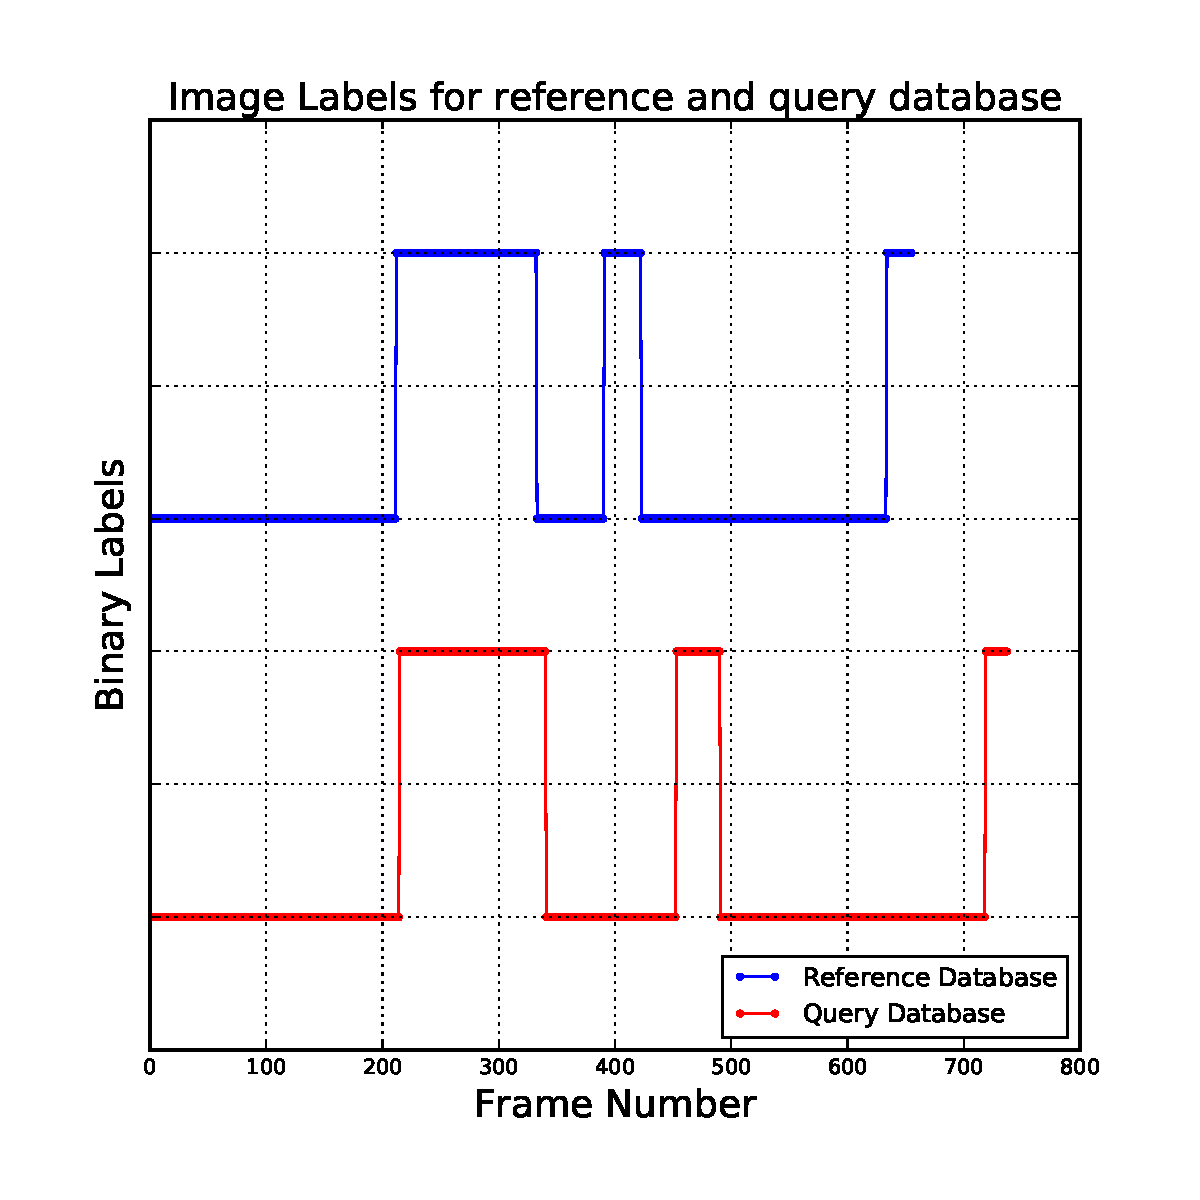
\includegraphics[scale=0.45]{cta-rail-imageLabels}
 \caption{Image Labels for reference and query database of CTA Rail dataset after post-processing of raw semantic labels.}
 \label{fig:datasetLabels}
\end{figure}


\subsubsection{Dataset Segmentation}
The filtered image labels of the reference database are used to segment the database into different chunks. These chunks represent the variation in appearance of the environment while traversing the route. For example, a train running underground as opposed to over ground will have different appearance of its environment. Similarly, a person walking indoor or outdoor of a campus will witness different surrounding environment as shown in figure\ref{fig:labelledImages}. This variation is therefore captured using the semantic labels of images and segmenting the image sequence into different regions. The segmented regions for one of the datasets used in this paper is shown in Figure \ref{fig:datasetLabels} for both reference and query database.

\subsection{Place Recognition}
\subsubsection{SeqSLAM}
SeqSLAM \cite{Milford2012} is a place recognition method known to work remarkably well in challenging environmental conditions. The recent advanced methods \cite{milford2015sequence}, \cite{wang2015improved}, \cite{milford2015place} etc. based on vanilla SeqSLAM further improve the state-of-the-art for place recognition. In this paper, we use the vanilla approach to show the performance improvement using semantic scene information. The detailed methodology of SeqSLAM can be referred to in \cite{Milford2012} and is briefly explained here. The method uses Sum of Absolute Difference (SAD) scores between preprocessed reference and query images. The preprocessing step involves down-sampling of image to $32\mathbf{x}32$ size and patch normalizing the images with a fixed window size $P$. The SAD matrix formed between the reference and query database undergoes contrast enhancement for each query image. The contrast enhancement refers to the normalization of SAD scores within a sliding window of size $R$. The contrast enhanced SAD matrix is then searched for image sequence trajectories of size $D_s$ within a limited range of velocities originating from each of the reference image. The sequence trajectory with best SAD score is then selected using a trajectory uniqueness threshold $\mu$.

\subsubsection{Segmented Region Normalization}
The contrast enhancement step in SeqSLAM uses an arbitrary window size for locally normalizing the matching scores as described above. We use the segmented regions of the dataset to set the normalization window of each query image. The label associated with the query image is used to identify the matching regions of dataset where the normalization is performed with window size equivalent to the size of the matching region. The unmatched regions use the vanilla method of contrast enhancement.

\section{Experimental Setup}
The experiments are performed using two datasets described in subsequent section. The image classification is performed using Dell M4800 Intel Core i7, 3.1 GHz processor with NVIDIA Quadro K2100M graphics card. The place recognition is performed using Dell E7450 Intel Core i7, 2.6 GHz processor. The classification is done as a preprocessing step for reference as well as query database off-line.

\subsection{Dataset}
The two datasets used in the experiments have instances of different environmental appearances as the route is traversed.

\subsubsection{CTA-Rail}
The CTA-Rail (Chicago Transit Authority) dataset comprises of two videos traversing a 23 km railway route (Blue Line to O'Hare) recorded once in 2014\cite {ctaRail2014} and then in 2015 \cite{ctaRail2015} available online. The video comprises of scenes from train stations platforms, subway station platforms, subway tunnels, railroad tracks within highways and urban areas. The entire video sequence captured at a high frame-rate is used for current experiments processing every 200th frame. The resultant reference and query database has 656 and 738 image frames respectively.

\subsubsection{Campus Indoor Outdoor}
The Campus Indoor Outdoor dataset comprises of two videos with repeated traversal of campus from outside lawn to inside corridor \cite{indoorOutdoor1,indoorOutdoor2}. The videos are recorded using a hand-held device and has jerky motion with huge motion blur. The raw videos are cropped to remove the comments at the bottom and an overlaid navigation display on the right side. The videos are also snipped from beginning so that the starting point is aligned in both the sequences. The dataset therefore comprises of scenes from outside the campus with trees, grass and field road, and from inside the campus traversing through entrance hall, staircase, lobby and corridor. The reference and query database is processed by using every 10th image and therefore uses 355 and 300 frames respectively.

\subsubsection{Ground Truth}
The place recognition ground truth for both the datasets is generated manually for intermittent frames and then interpolated for rest of the image sequence. A query image is considered to be a true positive match for the reference image if its index lies within a range of 5 image frames from the ground truth index.

\subsubsection{SeqSLAM parameters}
The parameters for SeqSLAM used for all the experiments are shown in Table \ref{table:seqSLAMParams}.

\begin{table}[!htbp]
 \begin{tabular}{|c|p{4cm}|p{2.5cm}|}
 \hline
  $S$ & Image Down-sampling Size & 32x32 \\
  \hline
  $P$ & Patch Normalization Window Size & {2,4,8,16} \\
  \hline
  $O$ & Image Matching Offset Range & $\pm10$ \\
  \hline
  $D_s$ & Sequence Length & 10 \\
  \hline
  $R$ & Contrast Enhancement Window Size & {10,20,40,80,160} \\
  \hline
  $V$ & Sequence Search Velocity Range & $1\pm0.4$ \\
  \hline
  $\mu$ & Trajectory Uniqueness Threshold & Varied from 0 to 255 \\
 \hline
 \end{tabular}
\caption{SeqSLAM parameters.}
\label{table:seqSLAMParams}
\end{table}


\section{Results}
The place recognition performance is measured using maximum F1 Score by varying the trajectory uniqueness parameter (described in \cite{Milford2012}), that is, the threshold for deciding a correctly matched place. We also varied two of the parameters of SeqSLAM method that are known to affect the performance, in order to understand the performance changes by using the proposed approach. The performance improvement is as shown in Figure \ref{fig:performanceChart} and the effect of parameters is discussed in subsequent section. 
\\
Figure \ref{fig:sadMat} shows the ground truth and the place recognition matches (without thresholding) corresponding to different parameter settings for both vanilla SeqSLAM and proposed method. The results in first row correspond to Campus Indoor-Outdoor dataset and second row to CTA Rail dataset. The performance improvement is large for both the datasets for smaller values of $R$ (contrast enhancement window size). The large $R$ values help the vanilla method to attain performance equivalent to the proposed approach as shown in Figure \ref{fig:sadMat}. The effect of dataset segmentation can be easily seen and understood in the result images in form of rectangular dark and light patches in the SAD matrix. 

\newcommand{\imgH}{5cm}
\newcommand{\imgW}{4cm}
\begin{figure*}[!htbp]
 \begin{tabular*}{\textwidth}{cccc}
  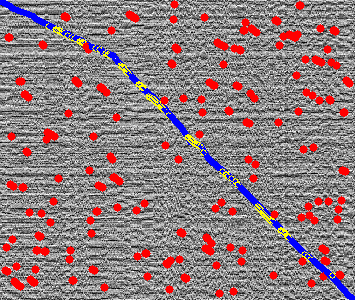
\includegraphics[width=\imgW,height=\imgH]{campus-io-without-bad-101} &
  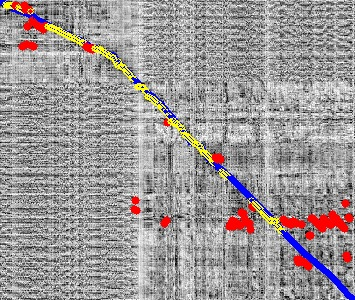
\includegraphics[width=\imgW,height=\imgH]{campus-io-with-bad-71} &
  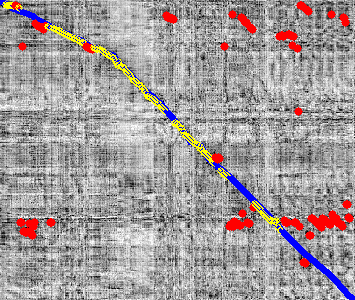
\includegraphics[width=\imgW,height=\imgH]{campus-io-without-good-105} &
  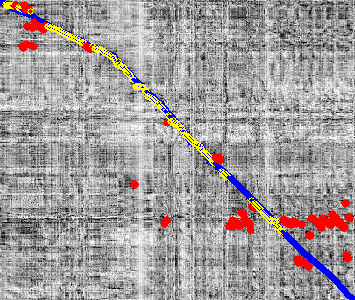
\includegraphics[width=\imgW,height=\imgH]{campus-io-with-good-75} \\
  (a) F Score = 0.46 & (b) F Score = \textbf{0.74} & (c) F Score = 0.72 & (d) F Score = \textbf{0.75} \\
  SeqSLAM & Proposed Approach & SeqSLAM & Proposed Approach \\
  \multicolumn{2}{c}{\textbf{R = 10}, P = 8} & \multicolumn{2}{c}{\textbf{R = 160}, P = 8} \\
  \multicolumn{4}{c}{\emph{Campus Indoor-Outdoor Dataset}} \\
  \\
  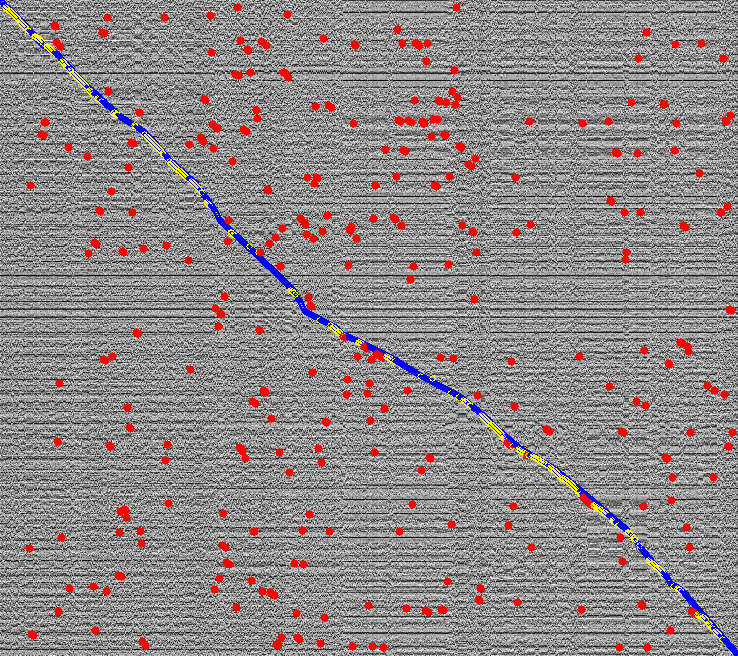
\includegraphics[width=\imgW,height=\imgH]{cta-rail-without-bad-106} &
  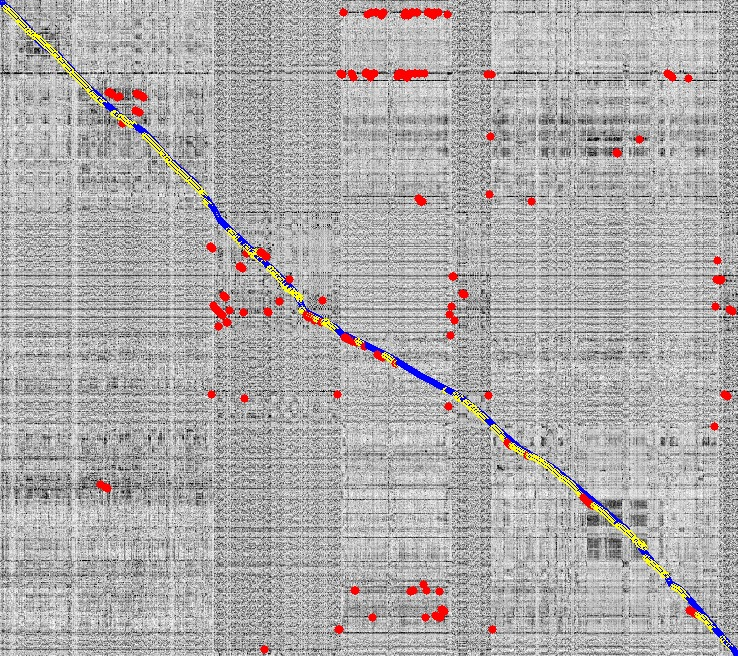
\includegraphics[width=\imgW,height=\imgH]{cta-rail-with-bad-306} &
  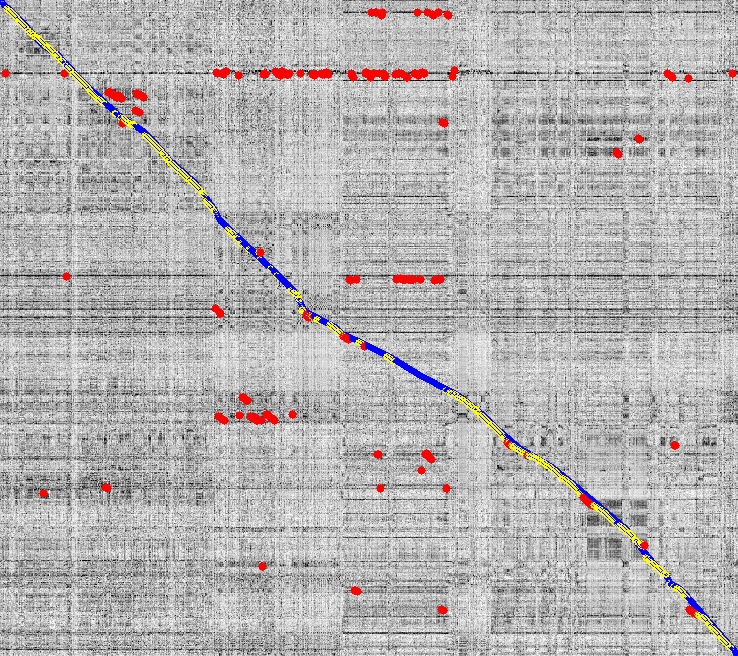
\includegraphics[width=\imgW,height=\imgH]{cta-rail-without-good-110} &
  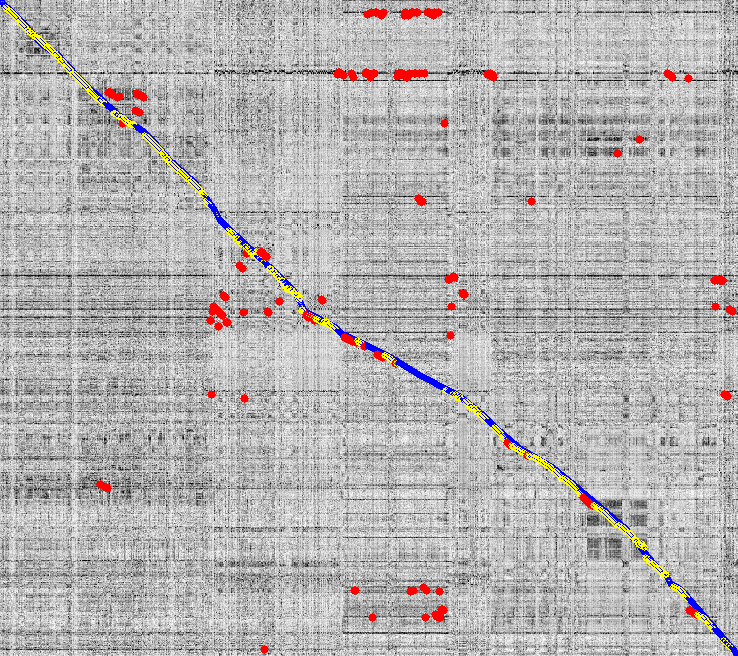
\includegraphics[width=\imgW,height=\imgH]{cta-rail-with-good-310} \\
  (e) F Score = 0.61 & (f) F Score = \textbf{0.82} & (g) F Score = 0.80 & (h) F Score = \textbf{0.82} \\
  SeqSLAM & Proposed Approach & SeqSLAM & Proposed Approach \\
  \multicolumn{2}{c}{\textbf{R = 10}, P = 4} & \multicolumn{2}{c}{\textbf{R = 160}, P = 4} \\
  \multicolumn{4}{c}{\emph{CTA Rail Dataset}} \\
 \end{tabular*}
 \caption{The SAD (Sum of absolute difference) matrix with reference database as rows and query database as columns. The ground truth is marked in blue, loop closures in red and true positives in yellow. The first and second row corresponds to Campus Indoor-Outdoor and CTA-Rail dataset respectively. Results in (a)-(b) and (e)-(f) correspond to smaller normalization window for vanilla SeqSLAM and proposed approach respectively while (c)-(d) and (g)-(h) correspond to larger normalization window. The dataset segmentation can be seen as rectangular dark and light patches. The images here show that performance improvement is large for smaller R values and with larger R values, performance of vanilla SeqSLAM method approaches to that of proposed method.}
 \label{fig:sadMat}

\end{figure*}


\section{Discussion}
\subsection{Effect of SeqSLAM parameters}
\subsubsection{Contrast Enhancement Window Size ($R$)}
This parameter is used to set the window size for locally enhancing the contrast of the match scores, that is, normalizing the score values in a local window. As shown in Figure \ref{fig:performanceChart}, for vanilla SeqSLAM method, the performance improves with increasing the value of this parameter. This is also expected because normalizing over a larger image sequence balances the overall variation in scores, but it leads to suppressing of place recognition corresponding to images which have low matching scores. On the other hand, using segmented regions to set the window size, effectively enhances the contrast of matching scores in appropriate regions and yields correct matching pairs. The performance is, therefore, most of the times better than the best achieved using vanilla approach. Moreover, setting the window size large is not appropriate for large datasets and long time navigation.

\subsubsection{Patch Normalization Window Size ($P$)}
The images used for finding SAD score are preprocessed by down-sampling them to the size of $32\mathbf{x}32$ and patch normalizing them in order to counter the change in appearance of their matching counterparts. Depending on the type of environment and corresponding imagery, the patch normalization window size can give different performance, but a higher value is usually recommended. In the experiments conducted here, we found that patch normalization window size of 4 and 8 for the given down-sampling image size gives a better performance.

\begin{figure*}[!htbp]
\centering
 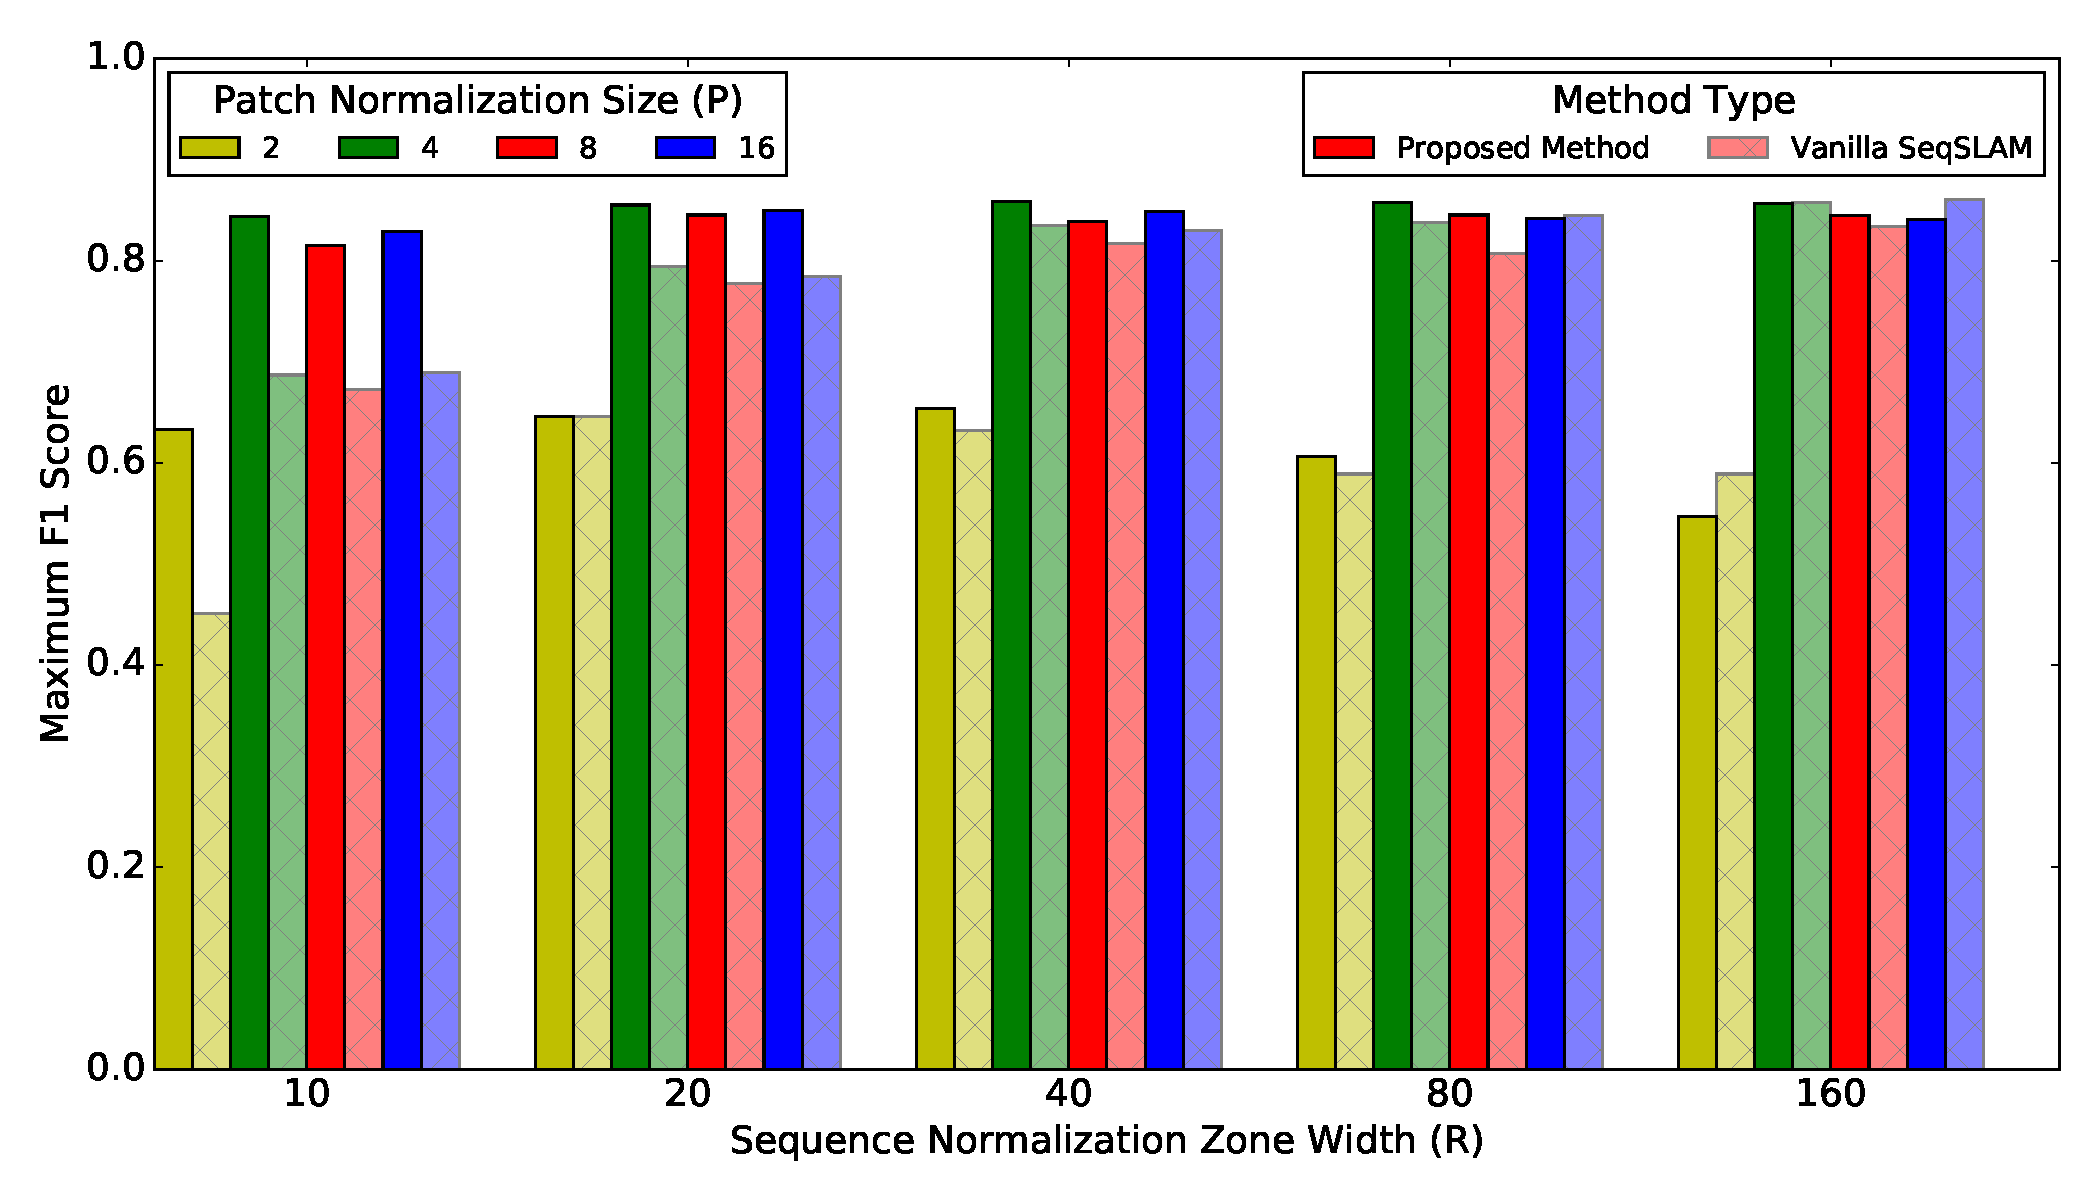
\includegraphics[scale=0.4]{cta-bar-graph} \\
 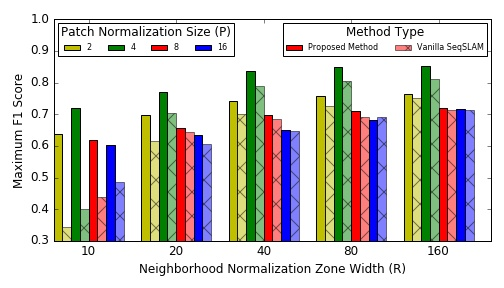
\includegraphics[scale=0.4]{campus-io-bar-graph}
 \caption{Performance chart showing maximum F1 Score. The first row corresponds to the CTA-Rail dataset and second row to the Campus Indoor-Outdoor dataset. The performance improves with increasing the parameter value R, where vanilla SeqSLAM performs equally good as the proposed approach. The patch normlization Size (P) parameter with value 4 tends to give maximum score as compared to others.}
 \label{fig:performanceChart}
\end{figure*}

\section{Conclusion}

\bibliography{ral-icra-2017}
\bibliographystyle{plain}

\end{document}
